\documentclass[a4paper,12pt]{report}

\usepackage[utf8]{inputenc}
\usepackage{graphicx}
\usepackage{geometry}
\geometry{left=1in,right=1in,top=1in,bottom=1in}
\usepackage{setspace}
\usepackage{longtable}
\usepackage{array}
\usepackage{booktabs}
\usepackage{caption}
\usepackage{multirow}
\usepackage{adjustbox}
\usepackage{rotating}
\usepackage{pdfpages}
\usepackage{amsmath}
\usepackage{xspace}
\usepackage{textcomp}
\usepackage{lscape}
\usepackage{amssymb}
\usepackage{bigstrut}
\usepackage{tcolorbox}

\setlength{\parindent}{0pt}
\renewcommand\thesection{\arabic{section}}

\begin{document}

\begin{center}
    
\includegraphics[width=4cm]{Figures/KhCE.png} \\
    \vspace{0.5cm}
    \textbf{(AN UNDERTAKING OF BHAKTAPUR MUNICIPALITY)}\\
    \vspace{0.5cm}
    \textbf{\LARGE KHWOPA COLLEGE OF ENGINEERING}\\
    \textbf{AFFILIATED TO TRIBHUVAN UNIVERSITY}
\end{center}

\vspace{1.5cm}
\begin{center}
    \textbf{\Large A}\\
    \textbf{\Large Report on}\\
    \vspace{0.5cm}
    \textbf{\large LAB 3: FIXED CAPACITOR THYRISTOR CONTROLLED REACTOR}\\[0.3cm]
\end{center}

\vspace{0.5cm}
\begin{center}
    \textbf{Submitted By : }
\end{center}

\begin{center}
    Shubhanga Aryal \qquad --------
\end{center}

\vspace*{1cm}
\begin{center}
    \textbf{Submitted To: }\\[0.2cm]
    \textbf{--------}\\[0.2cm]
    \textbf{-----------}
\end{center}

\vspace{0.3cm}
\begin{center}
\textbf{\Large Department of Electrical Engineering}\\
\vspace{0.3cm}
\textbf{KHWOPA COLLEGE OF ENGINEERING}\\
\vspace{0.3cm}
\textbf{Libali-08, Bhaktapur}
\end{center}

\thispagestyle{empty}
\newpage
\onehalfspacing
\begin{center}
    \Large{LAB 3}\\[0.2cm]
    \Large{FIXED CAPACITOR THYRISTOR CONTROLLED REACTOR}
\end{center}
\section{Objectives}
To understand the working of a fixed capacitor thyristor controlled reactor(FCTCR) 
and analyze the waveforms in MATLAB/Simulink.
\section{Software Used}
\begin{itemize}
    \item MATLAB/Simulink.
\end{itemize}
\section{Theory}
A basic VAR generator using a fixed capacitor with a thyristor controlled reactor is as shown in the Figure 1(a) below:
\begin{figure}[!hb]
    \centering
    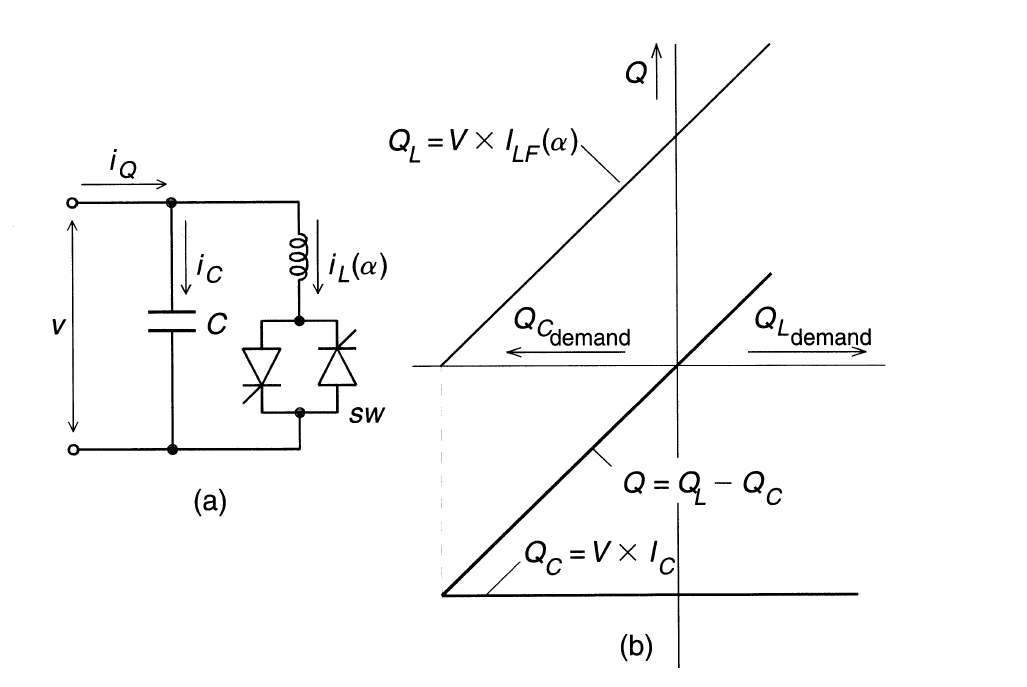
\includegraphics[width=0.7\textwidth]{Figures/figure1.png}
    \caption{Fixed Capacitor Thyristor Controlled Reactor}
    \label{Fig: FCTCR Circuit Diagram}
\end{figure}\\
The current in the reactor is varied similarly to the thyristor controlled reactor method. The FCTCR may be 
considered essentially to consist of a variable reactor (controlled by a delay angle $\alpha$) and a 
fixed capacitor. The constant capacitive var generation of the fixed capacitor is opposed by the variable var absorption ($Q_l$) of the thyristor controlled reactor to yield the total var output required as seen in Figure 1(b). At zero var output, the capacitive and inductive currents become equal and thus the capacitive and inductive vars cancel out. With a further decrease of angle $\alpha$ the inductive current becomes larger than the capacitive current, resulting in a net inductive var output. At zero var output, the capacitive and inductive currents become equal and thus the capacitive and inductive vars cancel out. With a further decrease of angle $\alpha$ the inductive current becomes larger than the capacitive current resulting in a net inductive var output. At zero delay angle, the thyristor controlled reactor conducts current over the full $180^\circ$ interval, resulting in maximum inductive var output that is equal to the var generated by the capacitor and those absorbed by the fully conducting reactor.\\[0.2cm]
When the inductive load decreases, the fixed capacitor will overcompensate. This overcompensation is neutralized reducing the firing angle of TCR branch with the help of a closed loop control system.
\section{Observation}
The circuit diagram to simulate the working of FCTCR is as shown in the figure below: 
\begin{figure}[!hb]
    \centering
    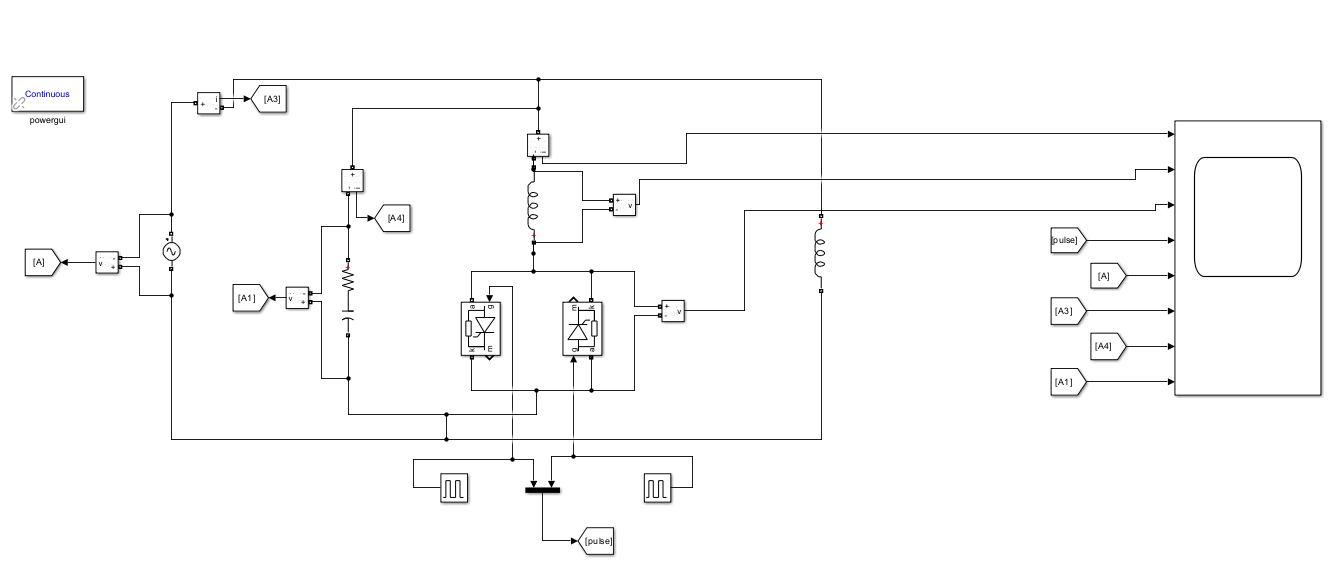
\includegraphics[width=1\textwidth,height=0.8\textwidth]{Figures/figure2.png}
    \caption{Simulation Model of FCTCR}
    \label{fig: Simulation Model}
\end{figure}\\
The observation was taken for $X_c>X_L$ for various firing angles and the value of \(X_C\) was 10e-3(F) where as the load inductor was 1e-3(H).\\
For $\alpha=90^\circ$:
\begin{figure}[!hb]
    \centering
    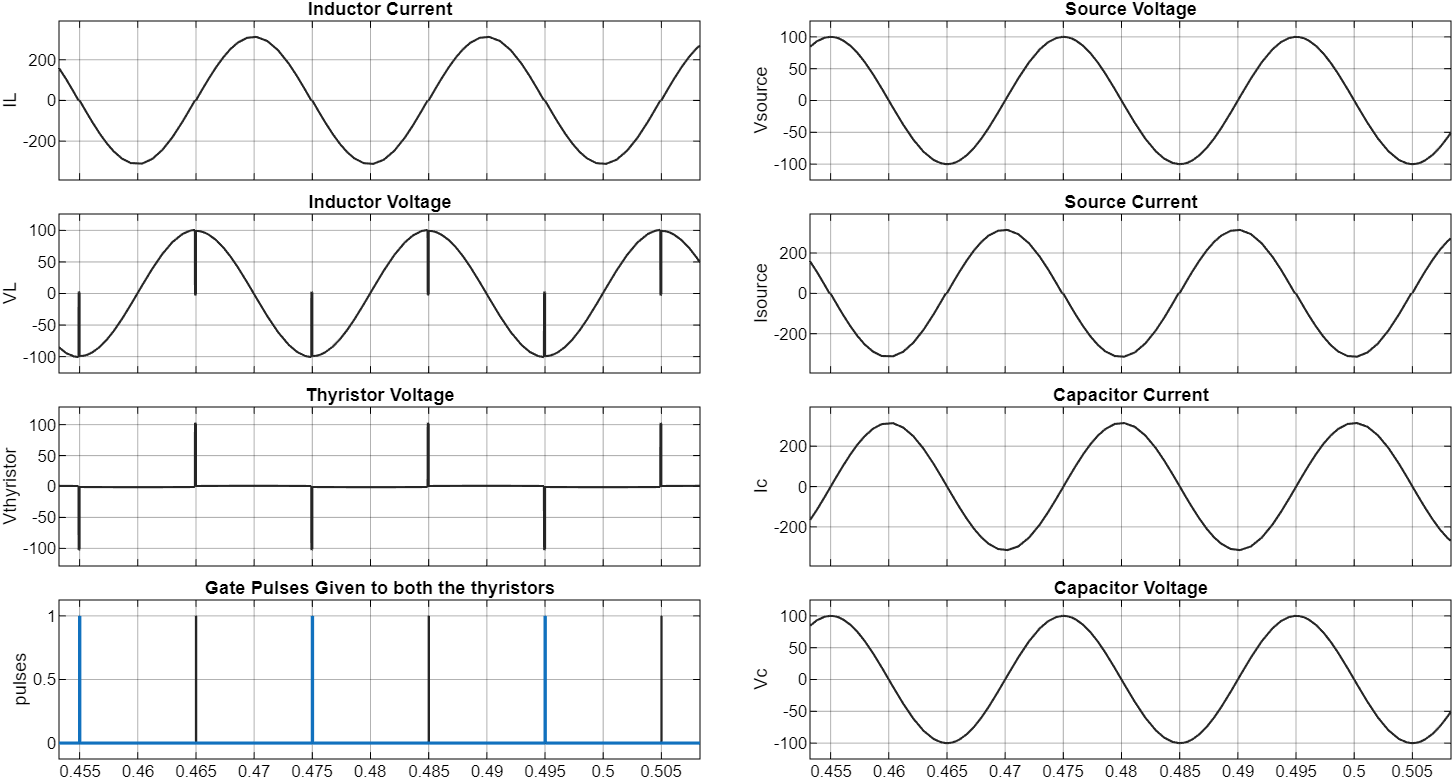
\includegraphics[width=1\textwidth]{Figures/figure3.png}
    \caption{FCTCR Waveforms for $\alpha=90^\circ$}
    \label{fig: FCTCR alpha 90}
\end{figure}\\
For $\alpha=120^\circ$:
\begin{figure}[!hb]
    \centering
    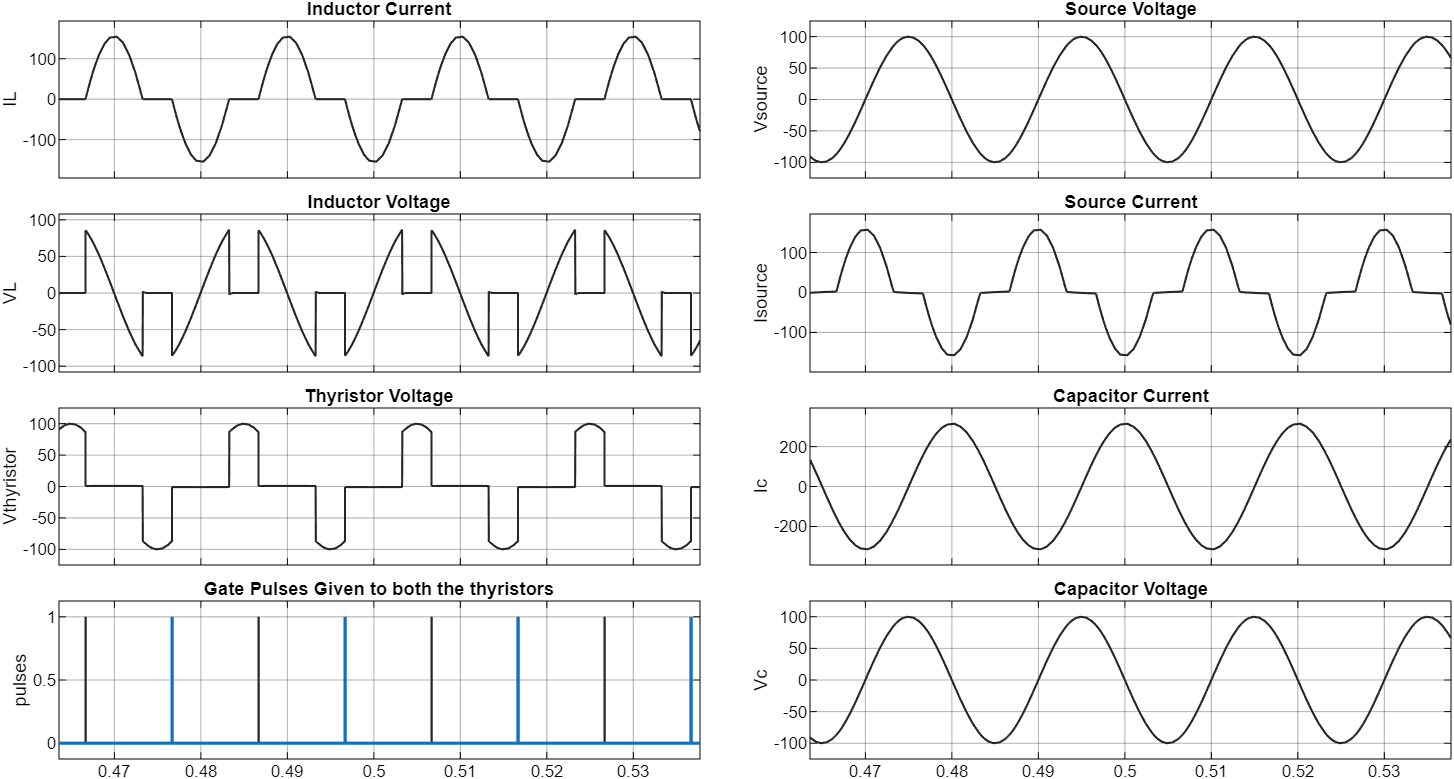
\includegraphics[width=1\textwidth]{Figures/figure4.png}
    \caption{FCTCR Waveforms for $\alpha=120^\circ$}
    \label{fig: FCTCR alpha 120}
\end{figure}\\
\newpage
For $\alpha=180^\circ$:
\begin{figure}[!hb]
    \centering
    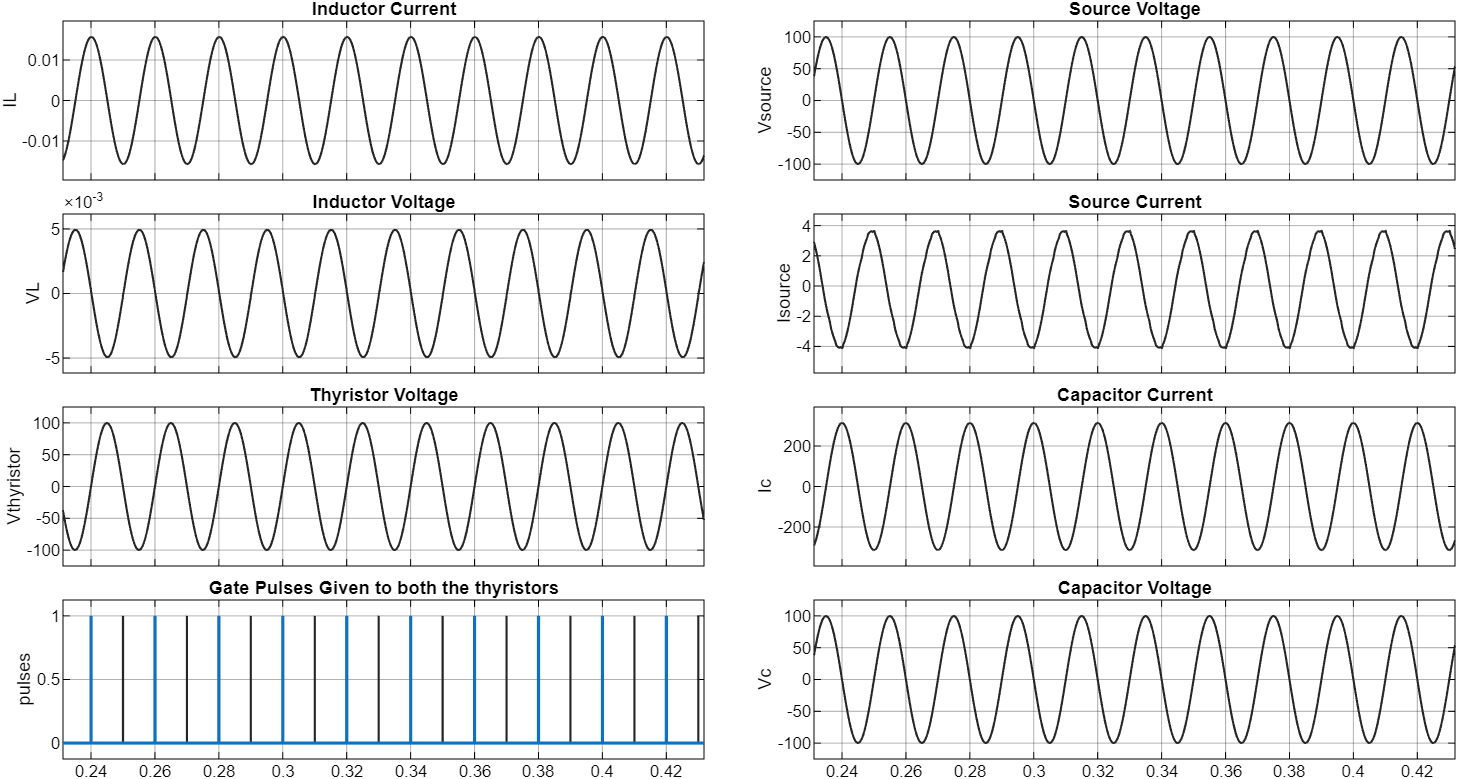
\includegraphics[width=1\textwidth]{Figures/figure5.png}
    \caption{FCTCR Waveforms for $\alpha=180^\circ$}
    \label{fig: FCTCR alpha 180}
\end{figure}\\
Same process was repeated for $X_L>X_C$ and observed for the same firing angle as before: 
For $\alpha=90^\circ$:
\begin{figure}[!hb]
    \centering
    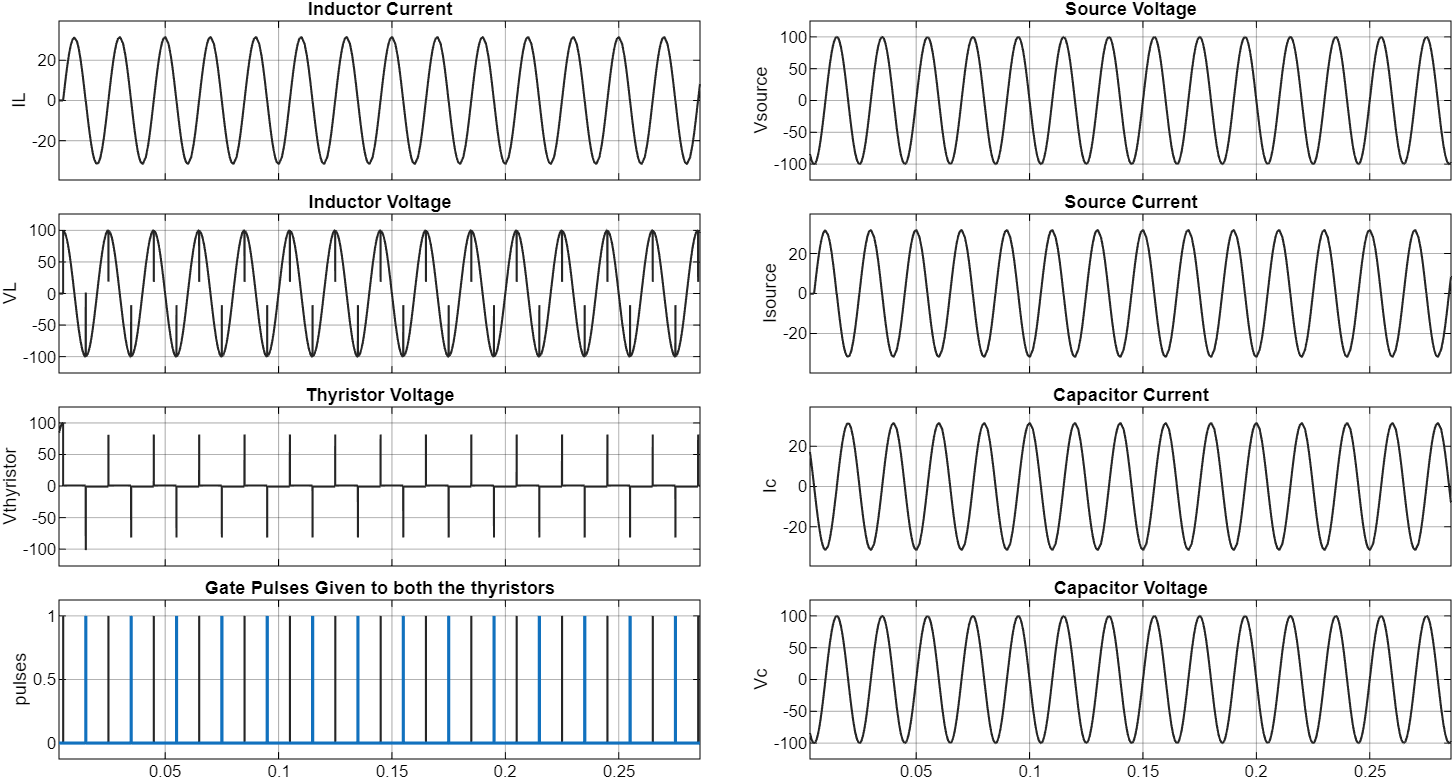
\includegraphics[width=1\textwidth]{Figures/figure6.png}
    \caption{FCTCR Waveforms for $\alpha=90^\circ$ ($X_L>X_C$)}
    \label{fig: FCTCR alpha 90 XL>XC}
\end{figure}\\
\newpage
For $\alpha=120^\circ$:
\begin{figure}[!hb]
    \centering
    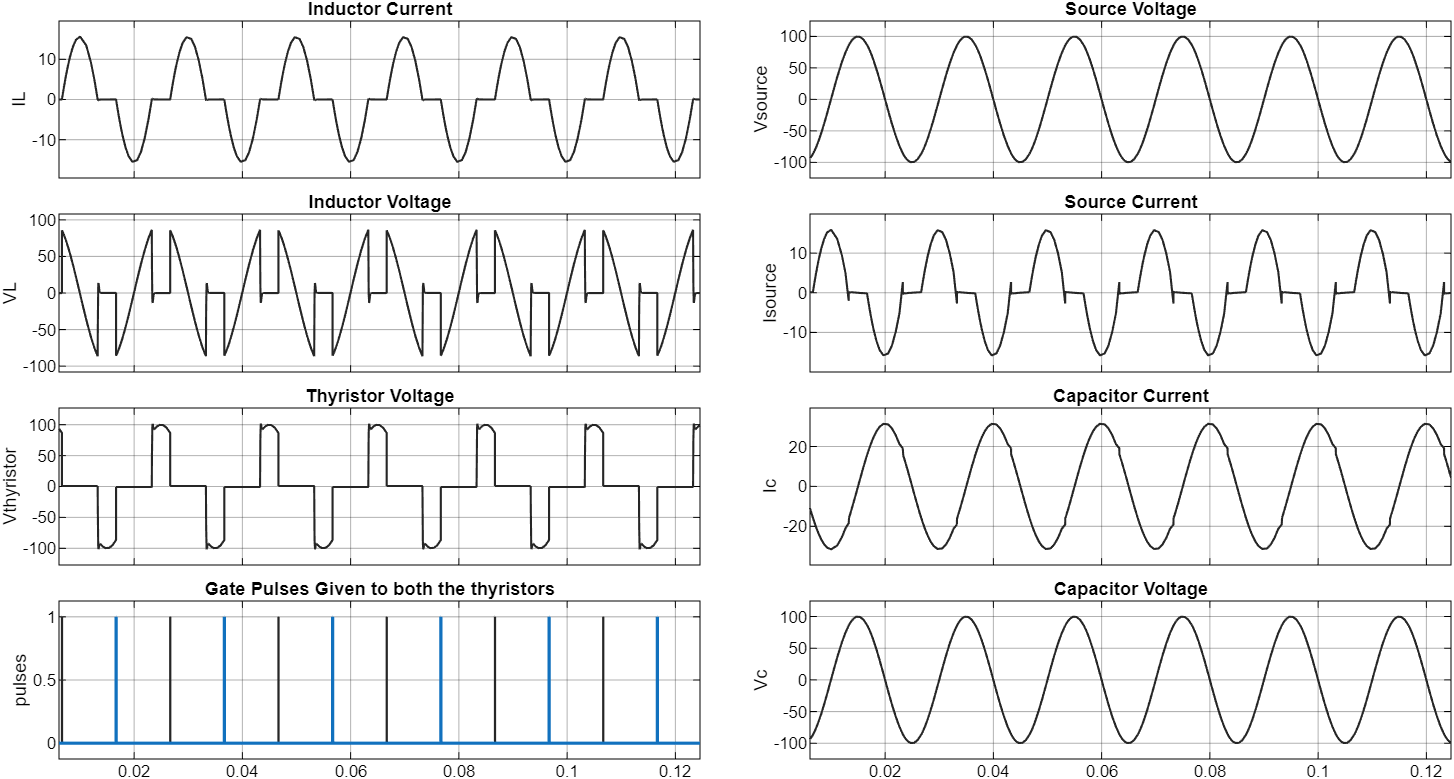
\includegraphics[width=1\textwidth]{Figures/figure7.png}
    \caption{FCTCR Waveforms for $\alpha=120^\circ$ ($X_L>X_C$)}
    \label{fig: FCTCR alpha 120 XL>XC}
\end{figure}\\
For $\alpha=180^\circ$:
\begin{figure}[!hb]
    \centering
    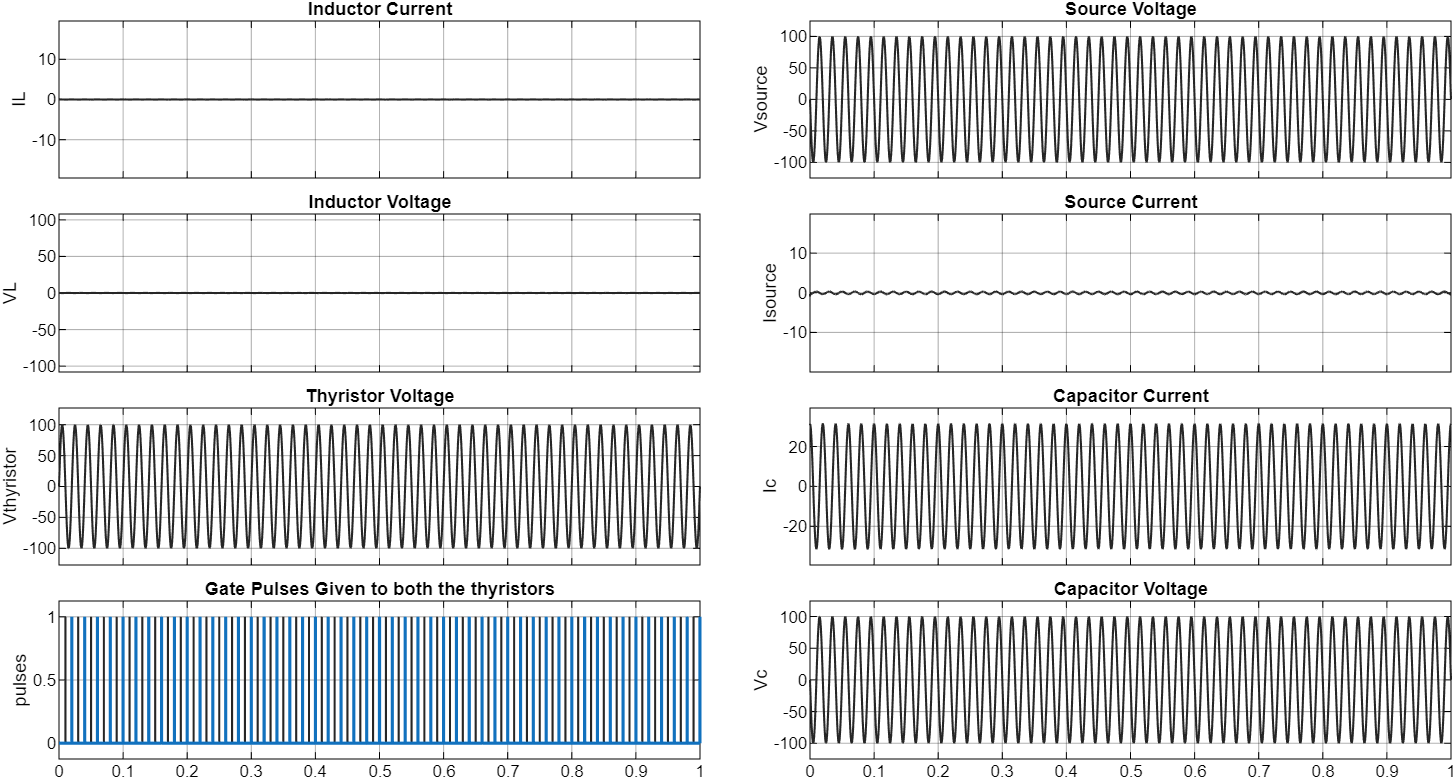
\includegraphics[width=1\textwidth]{Figures/figure8.png}
    \caption{FCTCR Waveforms for $\alpha=180^\circ$ ($X_L>X_C$)}
    \label{fig: FCTCR alpha 180 XL>XC}
\end{figure}
\newpage
\section{Discussion}
In this lab, we simulated the working of fixed capacitor thyristor controlled reactor for various firing angles and two conditions. At $alpha=90^\circ$ the thyristor pairs are fully conducting, and the scheme generated reactive power as shown in the figure. Between 90 and 180, we can see that the inductor current is leading with the source voltage and even at 180 degrees. Hence, we can say that the scheme generates reactive power.\\[0.2cm]
When inductive mode, the source current or the inductive current was greater than the capacitive current. And hence at 90 degrees the compensation current is purely sinusoidal and consumes reactive power. At 120 degrees, we can see that the compensating current is not sinusoidal and is still lagging with the source voltage. Hence, this scheme, consumes reactive power.\\[0.2cm]
However at 180 degrees, the thyristors are completely off and the inductor current and voltage are completely near equal to zero. In this case, in both the scheme it generates reactive power, which matches the theoretical expectation.
\section{Conclusion}
Thus, the working of FCTCR and its effect on different firing angles was simulated and understood.
\end{document}
